\section{IIR - Infinte Impulse Response}\label{sec:iir} 

    \subsection{Opbygning af Parametrisk Equalizer}


 
    \subsection{Design af filter}
    Parametre som brugeren skal kunne justerer: $\omega_0$ centerfrekvensen, $G$ forstærkning ved centerfrekvensen, $Q$ filterets godhed som bla. beskriver
    båndbredden på pasbåndet.\\
    Øvrige parametre:
    $G_0$ reference forstærkning (sættes til 1 for at kunne kaskadekoble flere bånd), $G_B$ forstærkning ved knækfrekvenserne (typisk 3dB over/under fra analog filterteori).
    
    Til at designe et IIR-filter bruges Bilinear transformations metoden (BLT).\\
    BLT består af følgende 3 trin:
    \begin{enumerate}
        \item Definer digital specifikationer og prewarp/frekvenswarp dem til analog specifikationer.$h(\omega) = h(\omega)|_{\omega = \Omega}$.
        \item Udfør analog filter design.
        \item Substituer BLT for at få det digitale filter. $H_a(s)|_{s = \frac{z^{-1} - 1}{z^{-1} + 1}} = H(z) $.
    \end{enumerate}
    
    Samplingsfrekvensen $f_s = \dfrac{1}{T_s}$

    \begin{align*}
    \omega_0 = \dfrac{2 \pi f_0}{f_s}
    \end{align*}
        \begin{align}
        \Delta \omega = \dfrac{\omega_0}{Q}
        \end{align}

    \subsection{Frekvenpreswarp}
    Da center frekvensen af filteret vil blive forskudt når der udføres en Bilinear
    transformation er det nødvendigt at prewarp'e (kompensere mod forvrængning), således at center frekvensen passer i det digitale filter.\\
    $\Omega_0$ er den analoge centerfrekvens, $\omega_0$ er den ønskede centerfrekvens, $f_s$ er samplingsfrekvensen. 
    Forholdet mellem $\Omega_0$ og $\omega_0$:


    \begin{align}
    \Omega = \tan\left(  \dfrac{\omega_0}{2} \right) 
    \end{align}

    \begin{align}
        \omega_0^2 = \omega_1 \cdot \omega_2 
    \end{align}
    \begin{align}
        \Delta \omega = \omega_2 - \omega_1
    \end{align}

    Heraf kommer et udtryk for den analog båndredde $\Delta \Omega$ i forhold til den ønskede båndredde $\Delta \omega$ og den analog center frekvens $\Omega_0^2$.
\begin{align}
    \tan \left( \dfrac{\Delta \omega}{2} \right) = \tan \left( \dfrac{\omega_2 - \omega_1}{2} \right) = \dfrac{\tan(\omega_2/2) - tan(\omega_1/2)}{1 + tan(\omega_1/2) \cdot tan(\omega_2/2)} = \dfrac{\Omega_2 - \Omega_1}{1 + \Omega_1 \Omega_2} = \dfrac{\Delta \Omega}{1 + \Omega_0^2}\\
    \iff \Delta \Omega = (1 + \Omega_0^2) \tan \left( \dfrac{\Delta \omega}{2} \right)
\end{align}


    \subsection{Analog filter}

    Som filter til equalizeren bruges high-shelf, low-shelf, peak/notch.
    Som filter bruges 2. orden da der i typisk ikke vil være brug for højere orden
     inde for audio. 



     \subsubsection{Peak/notch filter}


     Et peak/notch filter i en parametrisk equalizer består af et båndpas $H_{BP}$ og et båndstop $H_{BS}$ filter. Hvis
    $H_{band}$ repræsenterer det enkelte bånds overføringsfunktion.

    I ligning \ref{eq:band} summeres båndstop- og båndpasfilteret for kun
    at forstærke/dæmpe signalet omkring center frekvensen.\\
    Et analogt båndpas filter kan beskrives med ligning \ref{eq:bp_proto} 
    hvor $\alpha$ er en konstant der er afhængig af frekvensspecifikationer, $\Omega_0$ er centerfrekvensen.\\
    I ligning \ref{eq:bs_proto} er en overføringsfunktion for et båndstopfilter.


     \begin{align}
     H_{NOTCH}(s) = \dfrac{s^2 + \Omega_0^2}{s^2 + \alpha s + \Omega_0^2}
     \label{eq:lp_proto}
    \end{align}
    \begin{align}
      H_{PEAK} (s) = \dfrac{\alpha s}{s^2 + \alpha s + \Omega_0^2}  
    \end{align}

     \begin{align}
     H_a (s) = G_0 H_{NOTCH} (s) + G H_{PEAK} (s) = \dfrac{G_0 (s^2 + \Omega_0^2) + G \alpha s}{s^2 + \alpha s + \Omega_0^2}
     \label{eq:hp_proto}
    \end{align}

    \begin{align}
        G_B = \dfrac{G_0^2 + G^2}{2} \label{eq:gain_b}
    \end{align}

    Ved at sætte $s = j \Omega$ i ligning \ref{eq:lp_proto}, \ref{eq:hp_proto}
    og sætte $\big| H(j\omega)\big|^2 = G_B^2$, hvor $G_B^2$ er den ønsket forstærkning
    ved ønskede centerfrekvens $\Omega_0$, kan parameteren $\alpha$ findes for de givne specifikationer.. 
    
    \begin{align}
     |H_{a}(j \Omega)| = \dfrac{G_0 (\Omega_0^2- \Omega^2)+ j G \alpha \Omega}{-\Omega^2 + j \alpha \Omega + \Omega_0^2}   
    \end{align}

    \begin{align}
        |H_{a}|^2 = G_B^2 =  \dfrac{(\Omega_0^2- \Omega^2)^2 + G^2 \alpha^2 \Omega^2}{(\Omega_0^2-\Omega^2)^2 +\alpha^2 \Omega^2}   \iff \Omega^4 - \left(2 \Omega_0^2 + \dfrac{G^2- G_B^2}{G_B^2- G_0^2} \alpha^2 \right) \Omega^2 + \Omega_0^4 =0
    \end{align}
    
    
    \begin{align}
       \Delta \Omega^2 = (\Omega_2 - \Omega_1 ) = \dfrac{G^2 - G_B^2}{G_B^2 - G_0^2}  \alpha^2 \rightarrow \Delta \Omega = \sqrt{\dfrac{G^2 - G_B^2}{G_B^2 - G_0^2}} \alpha \iff \alpha = \sqrt{\dfrac{G_B^2-G_0^2}{G^2 - G_B^2 }} \Delta \Omega
    \end{align}


    \begin{align}
    \alpha \equiv \beta (1 + \Omega_0^2)  = \sqrt{\dfrac{G_B^2-G_0^2}{G^2 - G_B^2 }} \left( 1 + \Omega_0^2 \right) \tan \left( \dfrac{\Delta \omega}{2} \right) \\
    \iff \beta = \sqrt{\dfrac{G_B^2-G_0^2}{G^2 - G_B^2 }} \tan \left( \dfrac{\Delta \omega}{2} \right) \label{eq:beta}
    \end{align}


        \subsubsection{Bilinear Transformation}


    \begin{align}
    s =   \dfrac{z^{-1} - 1}{z^{-1} + 1}
    \end{align}

    \begin{equation}
    H_d(z) = H_a(S)\bigg|_{S = \frac{z^{-1} -1 }{z^{-1} + 1}}
    \end{equation}
   \begin{align}
    H(z) = H_a(s)\bigg|_{s = \frac{z^{-1} -1 }{z^{-1} + 1}} = 
    \dfrac{\left(\dfrac{G_0 + G \beta}{1 + \beta} \right)- 2 \left(\dfrac{G_0 cos( \omega_0)}{1 +\beta} \right)z^{-1} + \left(\dfrac{ G_0 - G \beta}{1 + \beta }\right) z^{-2}}{1 - 2 \left(\dfrac{cos(\omega_0)}{1 + \beta}\right)z^{-1} + \left( \dfrac{1 - \beta}{1 + \beta} \right) z^{-2}}
   \end{align}

   Hvor parametrende er $Q$, $G$, $f_0$. Heraf beregnes $w_0$ udfra ligning (),$\Delta \omega$ udfra ligning (), $\beta$ fra ligning (\ref{eq:beta}), $G_B$ beregnes fra ligning (\ref{eq:gain_b}).
   På figur (
       %\ref{fig:iir_peak}
       ) betragtes indflydelsen fra $Q$ når den varierer.

 \begin{figure}[h]
    \centering
         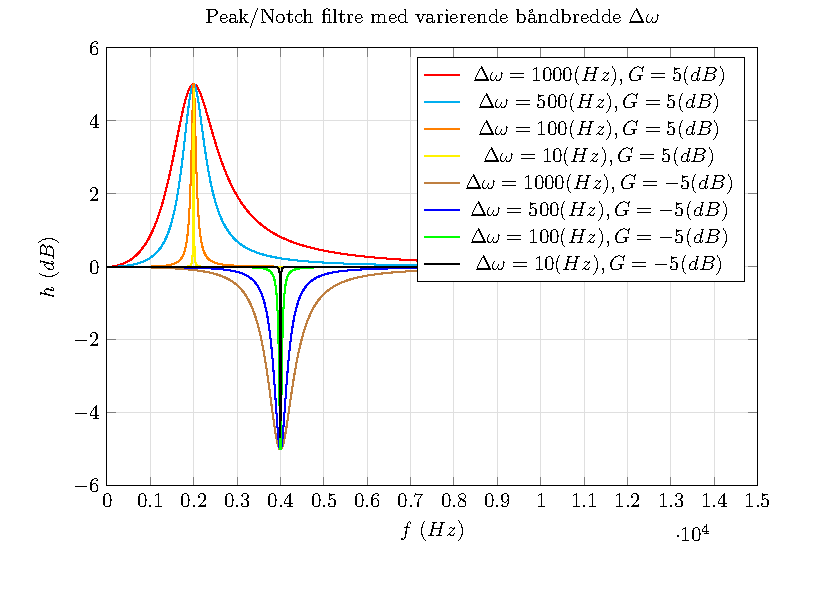
\includegraphics{figure/iir_peak.pdf}
        \caption{Peak/notch filtre med centerfrekvens $f_0 = 2kHz$ og $f_0 = 4kHz$, varierende $Q$ og gain $G=5dB$}
        \label{fig:iir_peak}
    \end{figure} 


     \subsubsection{Low-shelf filter}

   %  \begin{align}
    %     H_{LS}(z) = \dfrac{\sqrt{G} \left( \sqrt{G} \Omega^2 + \sqrt{2} \Omega G^{\frac{1}{4}} + 1 \right) +2 \sqrt{G} \left( \sqrt{G} \Omega^2 - 1\right) z^{-1} + \sqrt{G} \left(\sqrt{G} \Omega^2- \sqrt{2} \Omega G^{\frac{1}{4}} + 1 \right) z^{-2}}{\sqrt{G} + \sqrt{2} \Omega G^{\frac{1}{4}} + \Omega^2 + 2 \left( \Omega^2 - \sqrt{G} \right) z^{-1} + \left(\sqrt{G} -\sqrt{2} G^{\frac{1}{4}} + \Omega^2 \right) z^{-2}}
    % \end{align}

    Ved at sætte $\omega_0 = 0$ ind i ligning til peak/notch 
    filteret bliver det til et low shelf filter med knækfrekvensen $\omega_c$. 
    Forstærkningen ved knækfrekvensen $G_C$ defineres ligeledes $G_B$ i peak/notch filteret.
    Heraf kommer udtrykket for $\beta$ 
    \begin{align}
        H_a (s) = \dfrac{G_0 s + G \beta}{s + \beta}
    \end{align}

    \begin{align}
        |H_a (\Omega)|^2 = \dfrac{G_0^2 \Omega^2 + G^2 \beta^2}{\Omega^2 + \beta^2} = G_C^2
    \end{align}

    \begin{align}
        \beta = \sqrt{\dfrac{G_C^2 - G_0^2}{G^2 - G_C^2}} \tan \left( \dfrac{\omega_c}{2} \right)
    \end{align}

  
     \begin{align}
      H_{LS}(z) =   \dfrac{\left(\dfrac{G_0 + G \beta}{1 + \beta} \right)+ \left(\dfrac{ G_0 - G \beta}{1 + \beta }\right) z^{-1}}{1 + \left( \dfrac{1 - \beta}{1 + \beta} \right) z^{-1}}
     \end{align}

    \begin{figure}[h]
    \centering
        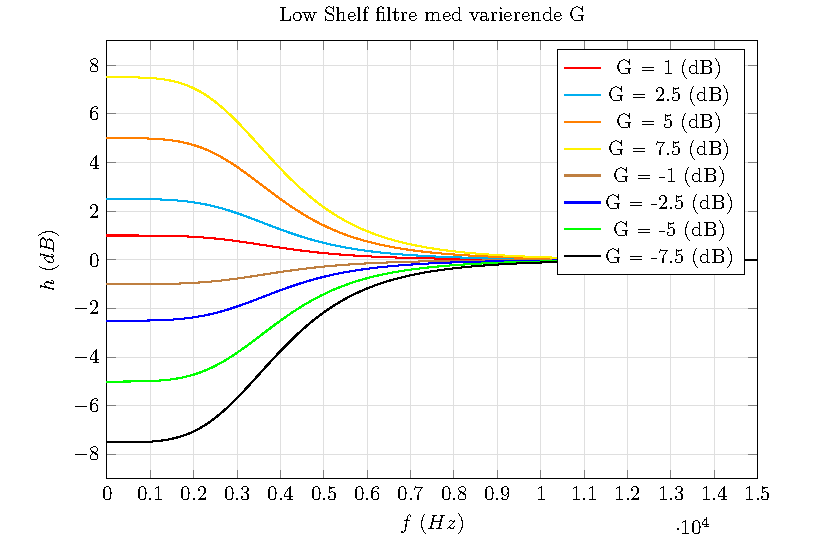
\includegraphics{figure/iir_ls.pdf}
        \caption{Low shelf filter med knækfrekvens $f_c = 4kHz$, varierende gain $G$ i intervallet: $[-7.5 ; 7.5]$}
    \end{figure} 
   
   
     \subsubsection{High-shelf filter}

     \begin{align}
        H_a (s) = \dfrac{G_0 + G \beta s}{1 + \beta s}
     \end{align}

     \begin{align}
         |H_a(\Omega)|^2 = \dfrac{G_0^2 + G^2 \beta^2 \Omega^2}{1 + \beta^2 \Omega^2} = G_C^2
     \end{align}
    \begin{align}
        \beta = \sqrt{\dfrac{G_C^2 - G_0^2}{G^2 - G_C^2}} \tan \left( \dfrac{\pi \omega_c}{2} \right)
    \end{align}

    %  \begin{align}
     %    H_{HS} = \dfrac{\sqrt{G} \left(  \sqrt{G} + \sqrt{2} \Omega G^{\frac{1}{4}}+ \Omega^2 \right) -2 \sqrt{G} \left( \sqrt{G} - \Omega^2 \right) z^{-1} + \sqrt{G} \left(\sqrt{G} - \sqrt{2} \Omega G^{\frac{1}{4}} + 1 \right) z^{-2} }{arg}
     %\end{align}

     Her indføres knækfrekvensen $\omega_c = \pi - w_0$ og $\omega_0 = \pi$ hvilket vil sætte centerfrekvensen i $f = \infty$, båndbredden bliver heraf knækfrekvensen 
     til HS filteret.

     $\beta$ beregnes med ligning (\ref{eq:beta}), hvorefter $cos(\omega_0) = cos(\pi) = -1$. Dette giver overføringsfuntionen HS filteret 
     der er en forkortet udgave peak/notch filtrenes overføringsfuntion.
     \begin{align}
     H_{HS}(z) =     \dfrac{\left(\dfrac{G_0 + G \beta}{1 + \beta} \right) + \left(\dfrac{ G_0 - G \beta}{1 + \beta }\right) z^{-1}}{1  + \left( \dfrac{1 - \beta}{1 + \beta} \right) z^{-1}}
     \end{align}


  \begin{figure}[h]
      \centering
        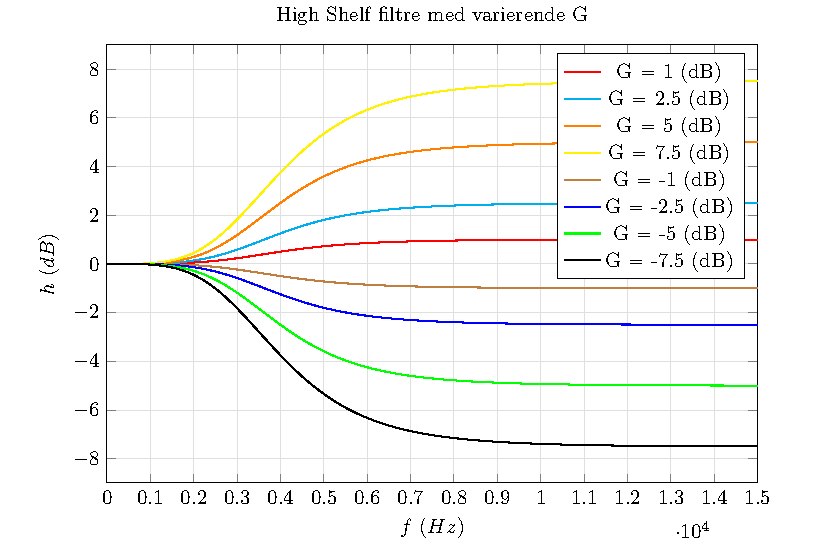
\includegraphics[]{figure/iir_hs.pdf}
        \caption{High shelf filter med knækfrekvens $f_c = 4kHz$, varierende gain $G$ i intervallet: $[-7.5 ; 7.5]$}
   \end{figure}  


 
  
 



 
    \subsection{Realisering af IIR-filter}

    Differensligning:
    \begin{align}
    y(n) = \sum\limits_{i=0}^{M} b_i x(n-i) - \sum\limits_{i=1}^N a_i y(n-i)
    \end{align}

   %\begin{figure}[h]
        %\centering
        %

\tikzstyle{dspsquare} = [shape=rectangle,draw=black,align=center,text depth=0.3em,text height=1em,inner sep=0pt,
	line cap=round,line join=round,line width=\dspblocklinewidth,minimum size=\dspsquareblocksize]
\tikzstyle{dspmultiplier} = [regular polygon, regular polygon sides=3,align=center,text depth=0.3em,
              text height=1em,inner sep=0mm,
              draw, fill=white, line width=\dspblocklinewidth,     
              shape border rotate=-90]
\tikzstyle{dspadder} = [circle,draw=black, line width=\dspblocklinewidth] 




\begin{tikzpicture}[]

\matrix[column sep=5mm, row sep= 1mm] at (0,0)
{
    %------------------------------------------------------- 
 \node[]               (m00)   {$x(n)$};        &
 \node[dspadder]         (m01)     {$+$} ;     &
 \node[coordinate]             (m02)   {}; &
 \node[coordinate]               (m03)   {};&
\node[coordinate]               (m04)      {}; &
 \node[dspmultiplier]    (m05)       {$ \quad b_0 $};         &
 \node[coordinate]               (m06)       {}; &
 \node[dspadder]         (m07)       {$+$};    &
 \node[]               (m08)        {$y(n)$}; \\ 
%------------------------------------------------------- 
 \node[coordinate]               (m10)       {};        &
 \node[coordinate]               (m11)       {}; &
 \node[coordinate]                (m12)  {}; &
 \node[coordinate]   (m13) {}; &
 \node[dspsquare]         (m14)       {$z^{-1}$};     &
\node[coordinate]        (m15)       {};         &
 \node[coordinate]               (m16)        {}; \\ 
%------------------------------------------------------- 
\node[coordinate]         (m20)       { };            &
\node[coordinate]         (m21)        {}; &
\node[coordinate]         (m22)        {}; &
\node[dspmultiplier,shape border rotate=90]  (m23)    {$-a_1$}; &
\node[coordinate]         (m24)       {};     &
\node[dspmultiplier]     (m25)       {$\quad b_1$};           &
\node[coordinate]       (m26)       { };             \\   
%------------------------------------------------------- 
\node[coordinate]         (m30)       { };            &
\node[coordinate]         (m31)        {}; &
\node[coordinate]         (m32)        {}; &
\node[coordinate]  (m33)    {}; &
\node[dspsquare]         (m34)       {$z^{-1}$};     &
\node[coordinate]      (m35)       {};           &
\node[coordinate]       (m36)       { };             \\  
%------------------------------------------------------- 
\node[coordinate]         (m40)       { };            &
\node[coordinate]         (m41)        {}; &
\node[coordinate]         (m42)        {}; &
\node[dspmultiplier,shape border rotate=90]  (m43)    {$-a_2$}; &
\node[coordinate]        (m44)       {};     &
\node[dspmultiplier]     (m45)       {$\quad b_2$};           &
\node[coordinate]       (m46)       { };             \\    
};

% 1. column
\draw [->] (m00) -- (m01);
\draw [->] (m01) -- (m05);
\draw [->] (m04) node[anchor = south west]{$w[0]$} -- (m14);
\draw [->] (m05) -- (m07);
\draw [->] (m07) -- (m08);
% 2. column
\draw [->] (m14) -- (m24) -- (m25);
\draw [->] (m24) node[anchor =south west]{$w[1]$} -- (m23);
% 3. column
\draw [->] (m24) -- (m34);
\draw [->] (m25) -- (m26) -- (m07);
\draw [->] (m23) -- (m22) -- (m01);

% 4. column
\draw [->] (m34) -- (m44) -- (m45);
\draw [->] (m44)  node[anchor=north west]{$w[2]$} -- (m43);
\draw [->] (m43) -- (m42) -- (m01);
\draw [->] (m45) -- (m46) -- (m07);
\end{tikzpicture}
    %    \caption{Realiserings diagram af 2. ordens iir filter. }    
    %\end{figure}

   

Kaskade form:\\

    
   \begin{align}
   H(z) = \prod\limits_{i=0}^{K-1} \dfrac{b_{i0} + b_{i1} z^{-1} + b_{i2} x^{-2}}{1 + a_{i1} z^{-1} + a_{i2} z^{-2}} 
   \end{align}


   Koefficienter:\\
   Koefficienterne haves i $K \times 3$ matricer hvor $K$ angiver antal bånd på equalizeren,
    $A_K$ er nævner polynomiet, $B_K$ er tæller polynomiet
   og $W_K$ er state-variablene.  


   \begin{align}
   A_{Kj} = \left[\begin{matrix}
   1 			& a_{01} 	& a_{02} \\
   1 			& a_{11} 	& a_{12} \\
   1 			& a_{21} 	& a_{22} \\
   \vdots 		& \vdots 	&  \vdots \\
   1 			& a_{K1} 	& a_{K2} \\
   \end{matrix}
   \right], \quad
      B_{Kj} = \left[\begin{matrix}
   b_{00}		& b_{01} 	& b_{02} \\
   b_{10}		& b_{11} 	& b_{12} \\
   b_{20}		& b_{21} 	& b_{22} \\
   \vdots 		& \vdots 	&  \vdots \\
   b_{K0}		& b_{K1} 	& b_{K2} \\
   \end{matrix}
   \right], \quad
      w_{Kj} = \left[\begin{matrix}
   w_{00}		& w_{01} 	& w_{02} \\
   w_{10}		& w_{11} 	& w_{12} \\
   w_{20}		& w_{21} 	& w_{22} \\
   \vdots 		& \vdots 	&  \vdots \\
   w_{K0}		& w_{K1} 	& w_{K2} \\
   \end{matrix}
   \right]
   \end{align}


